\documentclass[serif,9pt]{beamer}
\setbeamertemplate{navigation symbols}{}


\usetheme{Warsaw}

\usepackage[latin1]{inputenc}
\usepackage[spanish]{babel}


\beamersetuncovermixins{\opaqueness<1>{25}}{\opaqueness<2->{15}}

\begin{document}

\title[Virtualizaci�n en la educacion \ldots ]{Plataformas de virtualizacion para equipos en centros educativos}  
\author{Francisco Jos� Marin Cano \\ Jos� Maria Alcaraz Marin}
\institute[D.S.Y.C]{
  Departamento T�cnico de Sistemas y Comunicaciones\\
  Cieza (Murcia)}
\date{Copyleft \copyright{} 2013. Reproducci�n permitida bajo los \\
      t�rminos de la licencia de documentaci�n libre GNU.}

\section{Inicio}
\begin{frame}
\titlepage
\begin{center}

\includegraphics[scale=0.3]{albares1.jpg}
\end{center} 
\end{frame}

\section{Indice}
\begin{frame}\frametitle{Contenido}\tableofcontents
\end{frame} 


\section{Implantacion en IES Los Albares} 

\subsection{Temporalizacion}

\begin{frame}\frametitle{Linea de Tiempo}
\begin{center}
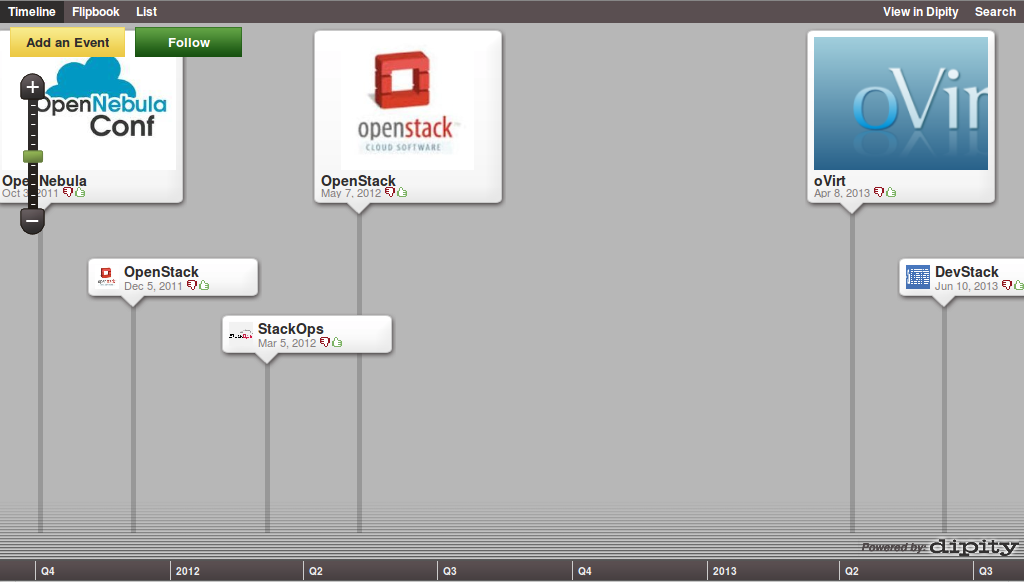
\includegraphics[scale=0.3]{TimeLine.png} 
\end{center}

\end{frame}


\subsection{Sistemas de virtualizacion utilizados}

\begin{frame}\frametitle{OpenNebula (Octubre 2011 - Noviembre 2011)} 
\begin{itemize}
\item El primer sistema que planteamos en utilizar fue OpenNebula, ya que este proyecto era muy ambicioso y prometia lo que se necesitaba.
\pause \bigskip
\item Instalamos una de las Primeras versiones, tras haber estado casi un mes peleandonos para poder configurar correctamente OpenNebula.
\pause \bigskip
\item Abortamos OpenNebula, ya que estaba en una fase temprana de desarrollo y aun faltaba mucho para que funcionara correctamente.
\end{itemize}


\end{frame}
\begin{frame}\frametitle{OpenStack (diciembre 2011 - Abril 2013 )}
\begin{itemize}
\item Nos costo mucho elegir despues de descartar OpenNebula, ya que habian muchos Sistemas de Virtualizacion, pero todos ellos estaban en un punto de Desarrollo muy temprano, ya que habian pocas funcionalidades y pocas de ellas funcionaban correctamente.
\pause \bigskip
\item Nos decidimos por OpenStack ya que estaba respaldada por un gran equipo de desarrolladores y detras estaba la NASA. Por lo que la parte de desarrollo seria mejor y mas rapida.
\pause \bigskip
\item Tambien ya que en el proyecto estaban varios centros, ellos tambien optaron por esta opcion con mejor o peor resultado.
\pause \bigskip
\item Como OpenStack esta en constante desarrollo optamos por dejar parado el proyecto hasta que saliera una version algo estable ya que cada poco tiempo cambian paquetes, configuraciones y demas, es decir lo que funcionaba un dia a la semana siguiente dejaba de funcionar y habia otra funcionalidad nueva.
\pause \bigskip
\item Por lo que este proyecto lo hemos dejado un poco en pausa hasta que salga una version estable y funcional.
\end{itemize}
\end{frame}
\begin{frame}\frametitle{StackOps (Marzo 2012 - Abril 2012)}
\begin{itemize}
\item Decidimos probar StackOps porque es una version de OpenStack pero con la personalizacion que introducen la gente de Ubuntu.
\pause \bigskip
\item Este sistema viene todo montado solo hace falta bajarse la iso e instalarla. Pero la configuracion es  Cero no deja modificar nada
\pause \bigskip
\item Lo probamos para ver como funcionaria un Sistema de Virtualizacion, aun asi seguian habiendo fallos en la interface visual y varios problemas que tambien estaban en OpenStack( ya que StackOps es un fork de OpenStack)
\end{itemize}
\end{frame}
\begin{frame}\frametitle{oVirt (Abril 2013 - Junio 2013}
\begin{itemize}
\item Es el ultimo que hemos estado probando y la verdad es que funciona bastante bien, eso si cuando funciona.
\pause \bigskip
\item Esta basado en RedHat por lo que en vez de instalar como para todos los anteriores Debian en este tubimos que instalar Feadora, aunque valdria cualquier distribucion basada en RedHat.
\pause \bigskip
\item El tema de configuracion es muy sencillo comparandolo con el de OpenStack.
\pause \bigskip
\item Una vez instalado y configurados los nodos de almacenamiento, hicimos una prueba intentando poner en funcionamiento varias maquinas virtuales Windows7
\pause \bigskip
\item Hasta aqui bien, el problema vino al apagar los nodos y el principal, cuando volvimos a arrancar he intentar iniciar las maquinas.
\pause \bigskip
\item oVirt nos decia en su interface web que el nodo de almacenamiento estaba bloqueado, tras varias pruebas e investigaciones llegamos a la conclusion que era un fallo de la plataforma y no lo habian solucionado todavia 
\end{itemize}
\end{frame}
\begin{frame}\frametitle{DevStack (Junio 2013 - ...)}
\begin{itemize}
\item Aunque conocimos de su existencia en los comienzos del proyecto, Ha sido ahora cuando lo hemos utilizado y nos hemos dado cuenta que falla tambien.
\pause \bigskip
\item DevStack es otro fork de OpenStack y lo que han conseguido esta gente es hacer el proceso de instalacion de OpenStack mas sencillo.
\pause \bigskip
\item Mediante su repositorio en github y configurando un par de scripts y completando unos ficheros de configuracion, puedes instalar tu Cloud
\pause \bigskip
\item Este es el ultimo que hemos probado y la verdad es que te ahorra muchisimo trabajo de configuracion con los scripts que incorpora.
\pause \bigskip
\item Lo instalamos correctamente e hicimos pruebas y hasta aqui todo bien, incluso tubimos arriba casi 20 maquinas virtuales, pero cuando reiniciamos el equipo donde instalamos DevStack dejo de funcionar.

\end{itemize}
\end{frame}

\subsection{Estado Actual}
\begin{frame}\frametitle{�Como se encuentra actualmente el proyecto?}
\begin{itemize}
\item El estado actual del proyecto esta un poco en el limbo ya que entre que no le podemos echar mucho tiempo ya que hasta ahora estabamos en practicas los horarios eran inconpatibles, y los problemas derivados del desarrollo, hasta que no se solucionen pues no se podra avanzar sobre este tema.
\pause \bigskip
\item Esperamos que muchos de los fallos que habian, se solucionen con las siguientes actualizaciones y con esto poder empezar la puesta en marcha del proyecto ya que es un proyecto ambicioso pero tambien esta en fase muy temprana de desarrollo por lo que habra que esperar un tiempo hasta que estas plataformas esten un poco mas consolidadas y fiables frente a errores comunes que son los que se dan actualmente.
\end{itemize}
\end{frame}



\section{Infraestructura necesaria para Virtualizaci�n}
\subsection{Computacion}
\begin{frame}\frametitle{Nodo Controlador}
\begin{itemize}
\item Supermicro-1012C-MRF Este equipo es el encargado de gestionar y organizar todo el cloud, es el que precisa una
mayor configuraci�n del software pero a su vez no requiere unas prestaciones elevadas.
Se ha optado por un servidor de una unidad de armario bastante convencional, en el que
se configurar�n los dos discos duros en modo RAID 1, para guardar los datos replicados en
previsi�n de futuros fallos de disco.
\pause \bigskip
\begin{itemize}
\item Chasis SC512F-350. Altura: 1U, anchura: 19", profundidad: 369 mm.
\item Placa base Supermicro H8SCM-F.
\item Fuente de alimentaci�n de 350W (80+ Gold).
\item 1 procesador AMD 4226 de 6 cores a 2700 MHz.
\item 4 GB de RAM DDR3/1333 ECC registrada
\item Dos interfaces de red Gigabit integradas Intel 82574L
\item Controladora Raid LSI 3 Ware 9650 SE ? 2LP de 128Mb PCI-E Raid 0,1 hardware.
\item 2 Discos duros internos de 500 GB SATA Seagate Constellation a 7200 rpm, 64MB de ca-
ch� e interfaz de 6G/s.
\item Interfaz de gesti�n IPMI 2.0

\end{itemize}

\end{itemize}
\end{frame}
\begin{frame}\frametitle{Nodo de Computacion (x4)}
\begin{itemize}
\item Supermicro-2022TG-H6RF Este equipo realmente son 4 equipos en 1, que comparten un mismo chasis y 2 fuentes de
alimentaci�n. Los 4 nodos de este equipo son totalmente independientes y cualquier fallo
en uno de ellos no afecta al funcionamiento de los dem�s. Estos 4 nodos son los equipos que realmente van a soportar la mayor parte del trabajo del
cloud, ya que en ellos se ejecutan todas las instancias del cloud (m�quinas virtuales)
\pause \bigskip
\begin{itemize}
\item Chasis 827HQ-R1620B. Altura: 2U, anchura: 19", profundidad: 724 mm.
\item 12 bah�as de 3.5" para discos duros extra�bles en caliente.
\item 4 placas base Supermicro H8DGT-HLF de doble socket AMD G34 y chipset AMD SR5690 +
SP5100.
\item 2 fuentes de alimentaci�n redundantes de 1620W (80+ Platinum).
\item 2 procesadores AMD 6238 de 12 cores a 2600 MHz o AMD 6220 de 8 cores a 3000 MHz
por nodo.
\item 32 � 64 GiB de RAM 1333 ECC registrada por nodo.
\item Dos interfaces de red Gigabit integradas Intel 82576 en cada nodo.
\item 1 tarjetas de red PCI-E de doble puerto Gigabit por nodo.
\item 2 Discos duros 350 GB SAS Seagate Cheetah a 15000 rpm, 16MB de cach� e interfaz de
6G/s por nodo.
\item 1 interfaz de gesti�n IPMI 2.0 por nodo.


\end{itemize}


\end{itemize}
\end{frame}
\subsection{Almacenamiento}
\begin{frame}\frametitle{QNAP TS-879U-RP}
\begin{itemize}
\item El QNAP TS-879U-RP, funciona como IP-SAN(iSCSI) y como NAS.
\pause \bigskip
\item La configuraci�n del acceso local o remoto con el TS-879U-RP es sencilla y no se necesitan conocimientos de TI. Todos los procesos de configuraci�n se han simplificado, de tal forma que la mayor parte del proceso es autom�tica o mediante un asistente de instalaci�n
\pause \bigskip
\begin{itemize}
\item Intel� Core? i3-2120 3.3GHz Dual Core
\item 2GB DDR3
\item Numero Max de Discos duros 8 x SATA(III)
\item Fuente de alimentacion 300W  Redundante
\item Consumo 68W/130W (sleep / trabajando)
\end{itemize}
\item Disponibles 8 teras de almacenamiento actualmente
\end{itemize}
 
\end{frame}
\subsection{Red}
\begin{frame}\frametitle{texto}

\end{frame}
\subsection{Energia}
\begin{frame}\frametitle{Sistema de Alimentacion Ininterrumpida}
\begin{itemize}
\item Para la infraestructura que se est� utilizando se ha optado por SAI de 2800 W y 4000 VA para soportar la carga de los distintos servidores y equipos de conectivi-
dad dedicados al proyecto.


\end{itemize}
\end{frame}
\section{Conetividad de los clientes}
\begin{frame}\frametitle{Como conectar con una maquina virtual}


\end{frame}
\end{document}

